\section{Blazor WebAssembly}

On the 6th of February 2018, Daniel Roth -- Program Manager on the ASP.NET team
at Microsoft -- released a blog post called \textit{A new experiment:
Browser-based web apps with .NET and Blazor}. In this post, \textcite{Roth_2018}
announces an experimental project from the ASP.NET team: a component-ori\"ented
web \gls{ui} framework based on C\#, .NET, HTML and so-called Razor pages. 

The promise that was outlined by this post was a way to enable developers to
write web applications using .NET technologies, rather than resorting to
Javascript\footnote{Javascript is an implementation of the ECMAScript
specification. Read more on \hrefself{https://ecma-international.org/tc39}}, the
primary scripting language used on the web.

Executing .NET binaries within a web browser is made possible by
\textbf{\gls{wasm}}\hreffootnote{https://webassembly.org/}, a binary instruction format.
\Gls{wasm} has been added to the \gls{w3c} recommendation list, and has become
the fourth language to run natively in web browsers, alongside HTML, CSS and
Javascript \autocite{Couriol_2019}. 

An overview of how Blazor works is provided in Figure~\ref{fig:blazor-wasm}.

Rather than \gls{transpiling} every .NET assembly to \gls{wasm}, or relying on
plugins, Blazor just relies on a .NET runtime that can run inside the browser
sandbox, just like regular Javascript does. The current implementation of Blazor
uses the \gls{wasm}-compiled version of the
Mono\hreffootnote{https://mono-project.com/} platform -- an open source .NET
runtime -- as an \gls{il} interpreter to execute managed code at runtime.

Because of this applications can leverage all standard web technologies like
websockets, the \gls{dom}, and all other browser \glsplural{api}, via
\textbf{\gls{jsinterop}}. It also ensures the various security protections put
in place by the sandbox environment to prevent malicious client-side attacks.

\begin{figure}
  \centering
  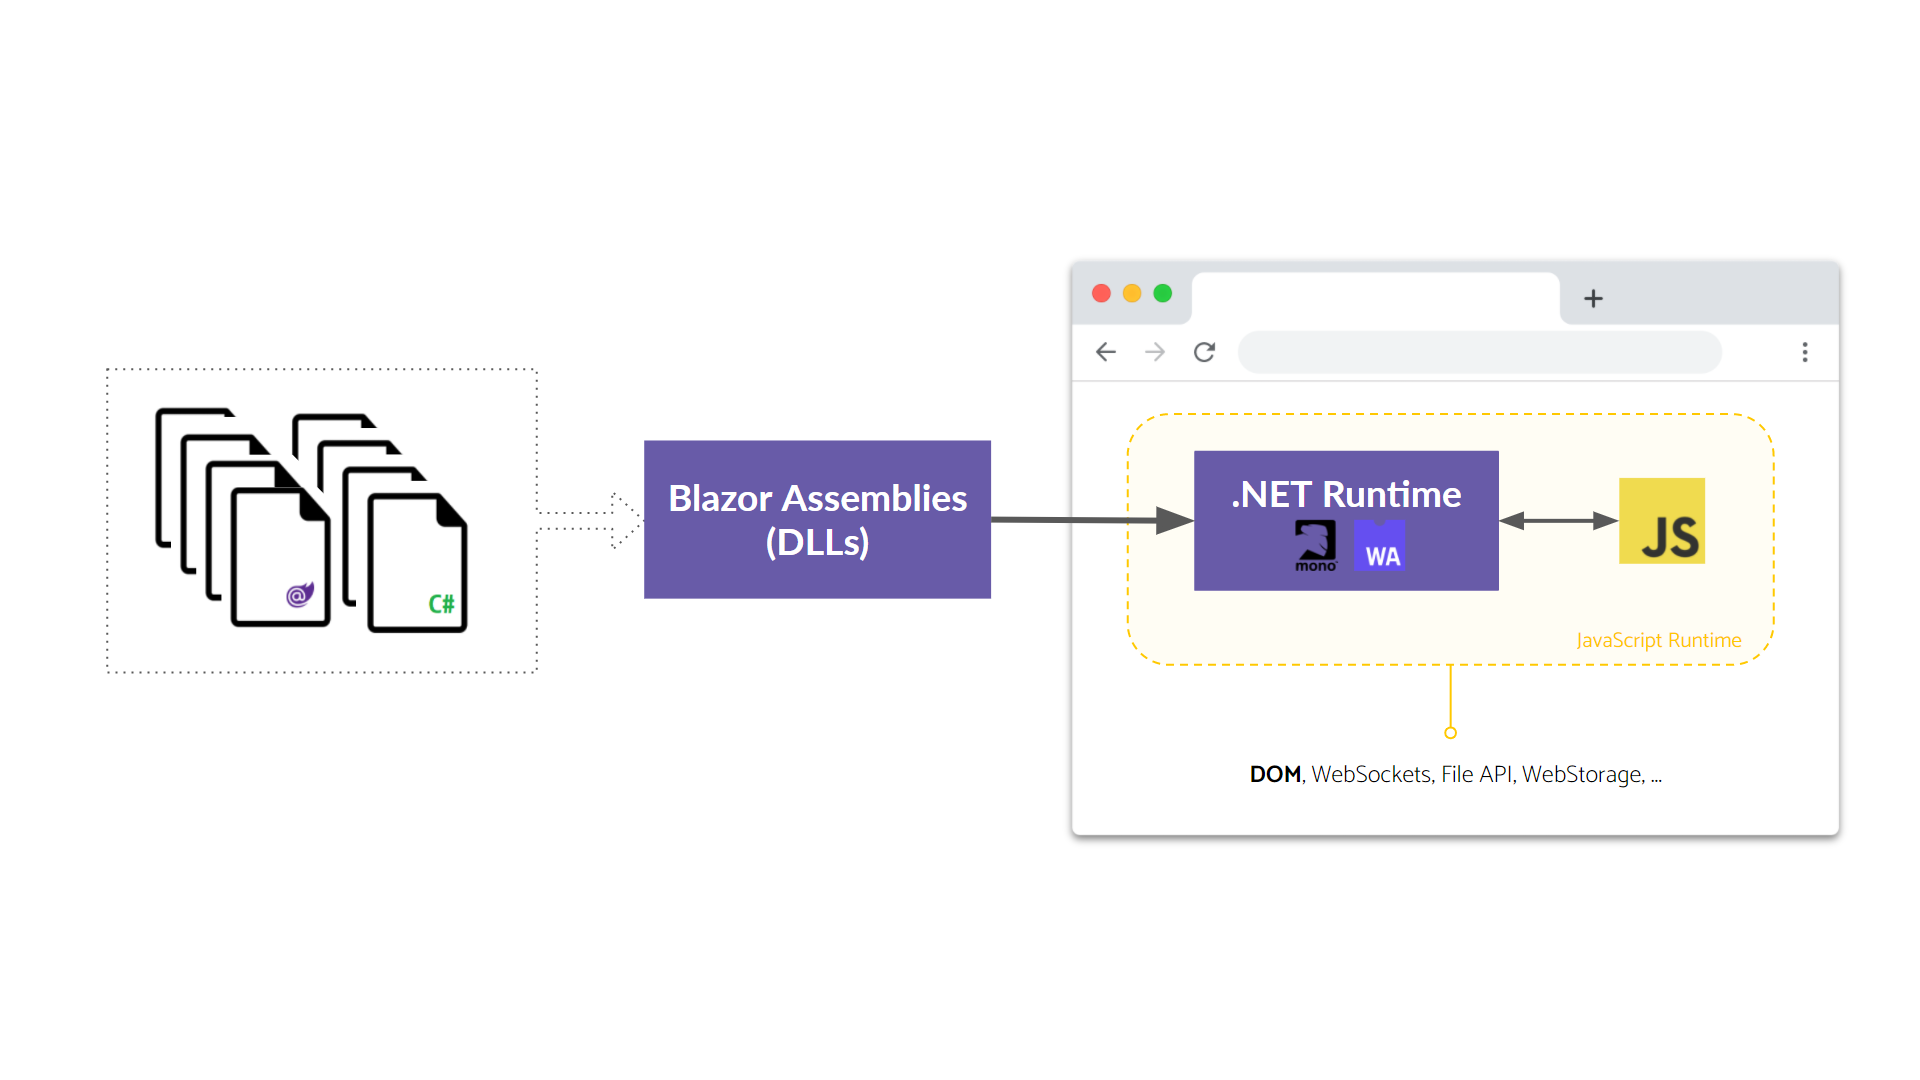
\includegraphics[width=0.8\textwidth]{blazor-wasm}
  \caption[Blazor WebAssembly]{A diagram that outlines how Blazor \gls{wasm}
  works. The C\# code and Razor files get compiled into \gls{il} assemblies, and
  run on a \gls{wasm} version of the Mono platform -- a .NET runtime -- inside
  the browser sandbox.}
  \label{fig:blazor-wasm}
\end{figure}


\subsection{Current state of Blazor and microfrontends}

According to \textcite{Rappl_MunichNETMeetup_2020}, an easy and effective way to
make distributed development possible in a Blazor WebAssembly project, is simply
to use separately distributed \textbf{component libraries}. In Blazor -- and in
the .NET ecosystem in general -- NuGet\hreffootnote{https://www.nuget.org} is
the standardized way of library distribution. One could create an \gls{appshell}
which imports and incorporates these NuGet packages. While this implementation
pattern makes development relatively straightforward, it has its downsides.

Because the integration happens at build-time; any change requires full
recompilation of the entire application. Also, upon startup, the \gls{appshell}
has to have full knowledge of all libraries, and they all have to be loaded for
the application to work, which makes this approach sub-optimal regarding
scalability. This integration method re-introduces coupling, and is generally
discouraged \autocite{Jackson_2019}.

Integrating \textbf{Blazor components in a JavaScript based app shell} is
another option. While this has been done succesfully\footnote{See an example
here: \hrefself{https://github.com/lauchacarro/MicroFrontend-Blazor-React}}, and
there are already some frameworks that support this idea\footnote{For example
the Piral microfrontend framework with their \texttt{piral-blazor} converter.
See \url{https://piral.io}}, it is not within the scope of this thesis, as the
focus is on an almost exclusive .NET-approach.

\subsubsection{Challenges and potential solutions}

When looking for an approach that can dynamically load assemblies at runtime,
the client-side \textbf{routing} starts to present a problem. When defining a
page component in Blazor, the \texttt{@page} directive can be used. This will
later provide the generated class with a \texttt{RouteAttribute} with a value
that indicates the component's desired route template. The standard Blazor
router will then use refletion on the specified \texttt{AppAssembly} to scan the
loaded assemblies for these \texttt{RouteAttribute}s \autocite{Sainty_2019}.
This starts to become an issue if the assemblies are dynamically loaded -- and
thus not present upon compilation. 

Another challenge that can present itself is \textbf{debugging}. When running
Blazor DLLs on a \gls{wasm} runtime, a mechanism is needed to provide the link
between the browser and the debugging tools: the debugging proxy. According to
\textcite{Abdalla_2020}, this is a seperate process that gets launched to load
so-called \gls{pdb} files. These are also called \textit{symbol} files, and they
are the link between the debugger and the source code \autocite{Microsoft_2021}.
Loading the \gls{microfrontend} symbol files dynamically is a challenge that
would need to be overcome to allow the debugging of Blazor applications using
\glsplural{microfrontend}.

These are challenges that would not come up when the composition would be done
at build-time like with component libraries. Luckily, the .NET 5 version of
Blazor introduces lazy-loading capabilities out of the
box\hreffootnote{https://docs.microsoft.com/en-us/aspnet/core/blazor/webassembly-lazy-
load-assemblies}, so most of these challenges that come from the dynamic loading
requirement can most likely be overcome. According to \textcite{Kdouh_2020}, the
Blazor router component, for example, now supports passing it additional
assemblies to consider. For debugging, the \texttt{AssemblyLoadContext} can
support the dynamic loading of dependencies with their symbols
\autocite{Microsoft_2019}. 